%%% LaTeX Template
%%% This template is made for project reports
%%%	You may adjust it to your own needs/purposes
%%%
%%% Copyright: http://www.howtotex.com/
%%% Date: March 2011

%%% Preamble
\documentclass[paper=a4, fontsize=11pt]{scrartcl}	% Article class of KOMA-script with 11pt font and a4 format
\usepackage[T1]{fontenc}
\usepackage{fourier}

\usepackage[english]{babel}															% English language/hyphenation
\usepackage[protrusion=true,expansion=true]{microtype}				% Better typography
\usepackage{amsmath,amsfonts,amsthm}										% Math packages
\usepackage[pdftex]{graphicx}														% Enable pdflatex
\usepackage{url}
\usepackage{graphicx}
\usepackage{hyperref}

%%% Custom sectioning (sectsty package)
\usepackage{sectsty}												% Custom sectioning (see below)
\allsectionsfont{\centering \normalfont\scshape}	% Change font of al section commands


%%% Custom headers/footers (fancyhdr package)
\usepackage{fancyhdr}
\pagestyle{fancyplain}
\fancyhead{}														% No page header
\fancyfoot[C]{}													% Empty
\fancyfoot[R]{\thepage}									% Pagenumbering
\renewcommand{\headrulewidth}{0pt}			% Remove header underlines
\renewcommand{\footrulewidth}{0pt}				% Remove footer underlines
\setlength{\headheight}{13.6pt}


%%% Equation and float numbering
\numberwithin{equation}{section}		% Equationnumbering: section.eq#
\numberwithin{figure}{section}			% Figurenumbering: section.fig#
\numberwithin{table}{section}				% Tablenumbering: section.tab#


%%% Maketitle metadata
\newcommand{\horrule}[1]{\rule{\linewidth}{#1}} 	% Horizontal rule

\title{
		%\vspace{-1in} 	
		\usefont{OT1}{bch}{b}{n}
		\normalfont \normalsize \textsc{University of Chicago Dept of Genetic Medicine} \\ [25pt]
		\horrule{0.5pt} \\[0.4cm]
		\huge PGRNseq Analysis \\
		\horrule{2pt} \\[0.5cm]
}
\author{
		\normalfont 								\normalsize
        Vassily Trubetskoy \\[-3pt]		\normalsize
        \today
}
\date{}


%%% Begin document
\begin{document}
\maketitle

\section{Overview}

Report on the analysis of sequence and chip data collected on 253 individuals undergoing chemotherapy with the drug Irinotecan.

\newpage

\section{Data}

	\subsection{Genotypes}

We currently have access to two different sets of genotypes for this population:
	
	\begin{enumerate}
		\item PGRNseq sequence data on VIP pharmacogenes.
		\item Illumina Exome Chip data. Run as an internal QC measure at the UW.
	\end{enumerate}
	
We have the alignment files for the sequence data. These were run through the consensus calling pipeline on Amazon.

	\subsection{Phenotypes}
	
The primary phenotype for this dataset is pharmacokinetic and pharmacodynamic data on patients. These PK/PD models are being generated at the University of North Carolina Chapel Hill.

In addition to PK/PD phenotypes, we are interested in looking at Neutropenia in patients. This is currently coded as the Neutrophil Count Nadir (NCN). This is defined as the lowest Neutrophil count observed in a patient during their course of therapy.

There are several relevant covariates available:
	\begin{itemize}
		\item site of collection
		\item sex
		\item drug dose
		\item self-reported ancestry
	\end{itemize}

	\subsection{Quality Control}
	Consensus calling in the sequence data. The results look very nice for the metrics that we have available (reference separate report, or put figures here).
	
	\begin{itemize}
		\item Exclude rare SNPs in single marker analyses
		\item Exclude SNPs out of HWE
		\item Exclude SNPs with high rates of genotype missingness
		\item Exclude SNPs with low QUAL
	\end{itemize}
	\subsection{Proposed Analyses}
	\begin{itemize}
		\item Linear regression. Using the estimated effect and its eror as a t-statistic. (GenABEL package in R)
		\item SKAT burden test. (SKAT package in R)
	\end{itemize}
	
	I'll have to think some more about which SKAT test is appropriate for this data.

\newpage

\section{Results}

	\subsection{Population Structure}
Sequence data provides too few variants to adequately identify ancestry through PCA .

The Exome chip data \emph{does} provide enough markers to differentiate samples. The spatial axes are well defined (see \hyperref[exomeAncestry]{Fig 3.1}). These PC's were used to identify a set of genetically homogenous samples (see \hyperref[exomeCluster]{Fig 3.2} and \hyperref[exomeCEUZoom]{Fig 3.3}).

%%% FIGURES
\begin{figure}[exomeAncestry]
\centering
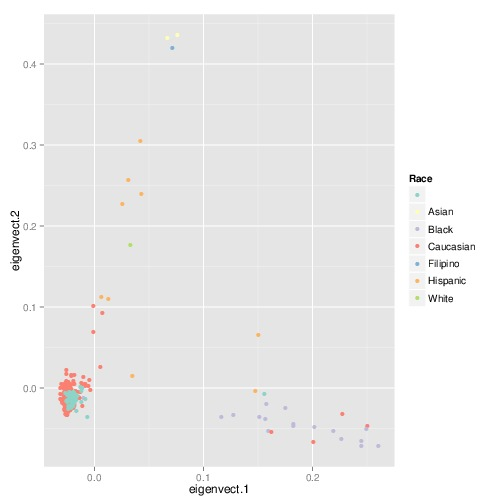
\includegraphics[scale=1.0]{{{plots/exomeChip.PCA.selfReportedAncestry}}}
\caption{First two principal components of exome chip genotype data. The samples segregate fairly well into their self-reported ancestries.	}
\end{figure}

\begin{figure}[exomeCluster]
\centering
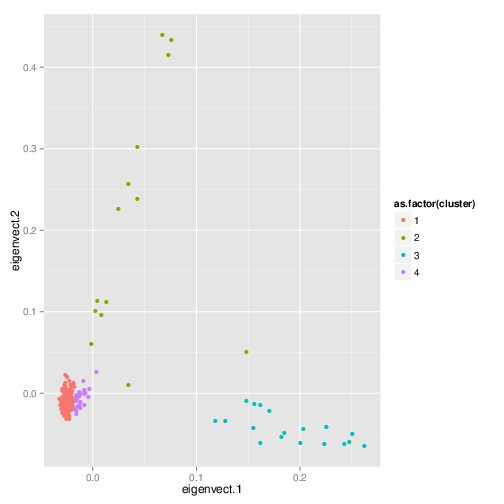
\includegraphics[scale=1.0]{{{plots/exomeChip.PCA.clustering}}}
\caption{Model based clustering of the first two pricipal components using the exome chip genotypes. These clusters were used to select a homogenous set of samples. In this case, we subset our data to the 161 samples contained in cluster 1.}
\end{figure}

\begin{figure}[exomeCEUZoom]
\centering
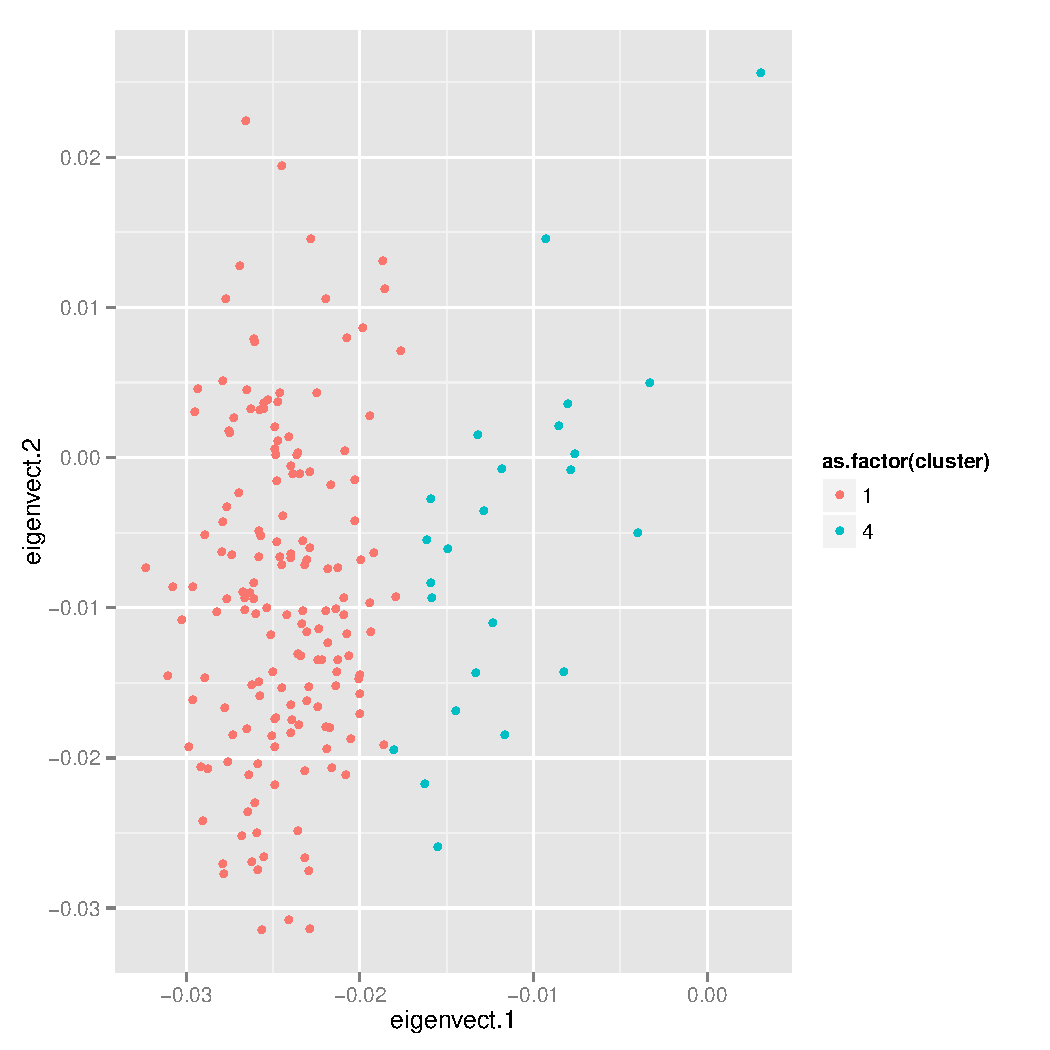
\includegraphics[scale=1.0]{{{plots/exomeChip.PCA.clustering.CEUzoom}}}
\caption{A zoom of the European cluster in the exome chip PCA. This shows some substructure, and we ultimately subset the samples contained in cluster 1.}
\end{figure}

	\subsection{Single Marker}
		\subsubsection{GenABEL Linear Regression}
		No results in sequence data for common variants.
		One significant results in Exome chip data
	\subsection{Gene-based}
		\subsubsection{Notes and Issues}
		The variants need to be cleaned. Right now, a lot of genes are dropped due to high rates of missingness. Additionally, many genotypes are being imputed through the SKAT package based on HWE.
		
		I am not using the small sample correction that the author's suggest for $n<2000$. P-values are computed with a parametric bootstrap with $n=10000$ iterations.
		\subsubsection{SKAT Burden}
		Currently running for the model: ANC ~ sex + site + dose. 11 samples are excluded for having missing covariate information.
		
		\subsubsection{SKAT Rare + Common}
		Very similar to the Burden. Top genes are the same with different p-values. 11 samples are excluded for having missing covariate information.

\section{References}


%%% End document
\end{document}
